
\documentclass[12pt]{beamer}\usepackage[]{graphicx}\usepackage[]{color}
% maxwidth is the original width if it is less than linewidth
% otherwise use linewidth (to make sure the graphics do not exceed the margin)
\makeatletter
\def\maxwidth{ %
  \ifdim\Gin@nat@width>\linewidth
    \linewidth
  \else
    \Gin@nat@width
  \fi
}
\makeatother

\definecolor{fgcolor}{rgb}{0.345, 0.345, 0.345}
\newcommand{\hlnum}[1]{\textcolor[rgb]{0.686,0.059,0.569}{#1}}%
\newcommand{\hlstr}[1]{\textcolor[rgb]{0.192,0.494,0.8}{#1}}%
\newcommand{\hlcom}[1]{\textcolor[rgb]{0.678,0.584,0.686}{\textit{#1}}}%
\newcommand{\hlopt}[1]{\textcolor[rgb]{0,0,0}{#1}}%
\newcommand{\hlstd}[1]{\textcolor[rgb]{0.345,0.345,0.345}{#1}}%
\newcommand{\hlkwa}[1]{\textcolor[rgb]{0.161,0.373,0.58}{\textbf{#1}}}%
\newcommand{\hlkwb}[1]{\textcolor[rgb]{0.69,0.353,0.396}{#1}}%
\newcommand{\hlkwc}[1]{\textcolor[rgb]{0.333,0.667,0.333}{#1}}%
\newcommand{\hlkwd}[1]{\textcolor[rgb]{0.737,0.353,0.396}{\textbf{#1}}}%
\let\hlipl\hlkwb

\usepackage{framed}
\makeatletter
\newenvironment{kframe}{%
 \def\at@end@of@kframe{}%
 \ifinner\ifhmode%
  \def\at@end@of@kframe{\end{minipage}}%
  \begin{minipage}{\columnwidth}%
 \fi\fi%
 \def\FrameCommand##1{\hskip\@totalleftmargin \hskip-\fboxsep
 \colorbox{shadecolor}{##1}\hskip-\fboxsep
     % There is no \\@totalrightmargin, so:
     \hskip-\linewidth \hskip-\@totalleftmargin \hskip\columnwidth}%
 \MakeFramed {\advance\hsize-\width
   \@totalleftmargin\z@ \linewidth\hsize
   \@setminipage}}%
 {\par\unskip\endMakeFramed%
 \at@end@of@kframe}
\makeatother

\definecolor{shadecolor}{rgb}{.97, .97, .97}
\definecolor{messagecolor}{rgb}{0, 0, 0}
\definecolor{warningcolor}{rgb}{1, 0, 1}
\definecolor{errorcolor}{rgb}{1, 0, 0}
\newenvironment{knitrout}{}{} % an empty environment to be redefined in TeX

\usepackage{alltt}
% only 10,11, or 12 pt fonts
% PACKAGES-----------------------------------
\usepackage{graphicx} % Allows including images
\usepackage{booktabs} % Allows the use of \toprule, \midrule and \bottomrule in tables

% THEMES AND COLORS-------------------------
\mode<presentation> {
\usefonttheme{default}
% FONTTHEMES: default, structurebold, structuresmallcapsserif, structureitalicserif, serif, professionalfonts


\usetheme{Warsaw}
% THEMES: default, AnnArbor, Antibes, Bergen, Berkeley, Berlin, Boadilla, boxes, CambridgeUS, Copenhagen, Darmstadt, Dresden, Frankfurt, Goettingen, Hannover, Ilmenau, JuanLesPins, Luebeck, Madrid, Malmoe, Marburg, Montpellier, PaloAlto, Pittsburgh, Rochester, Singapore, Szeged, Warsaw

\usecolortheme{crane}
%COLORTHEMES: default, albatross, beaver, beetle, crane, dolphin, dove, fly, lily, orchid, rose, seagull, seahorse, sidebartab, structure, whale, wolverine 

% DISPLAY OPTIONS--------------------------
%\setbeamertemplate{footline} % To remove the footer line in all slides, uncomment this line

%\setbeamertemplate{footline}[page number] % To replace the footer line in all slides with a simple slide count, uncomment this line

%\setbeamertemplate{navigation symbols}{} % To remove the navigation symbols from the bottom of all slides, uncomment this line
}
% -----------------------------------------



% TITLE PAGE DATA--------------------------


\setbeamercolor{normal text}{fg=black,bg=red}

\title[The Long Road]{The Chase} % The short title appears at the bottom of every slide, the full title is only on the title page

\author{Daniel Forcade} % Your name

\institute[UVM] % Your institution as it will appear on the bottom of every slide, may be shorthand to save space
{
University of Vermont \\ % Your institution for the title page
\medskip
\textit{daniel.forcade@uvm.edu} % Your email address
}
\date{\today} % Date, can be changed to a custom date or \today
% -----------------------------------------



% BEGIN DOCUMENT---------------------------
\IfFileExists{upquote.sty}{\usepackage{upquote}}{}
\begin{document}

{
\usebackgroundtemplate{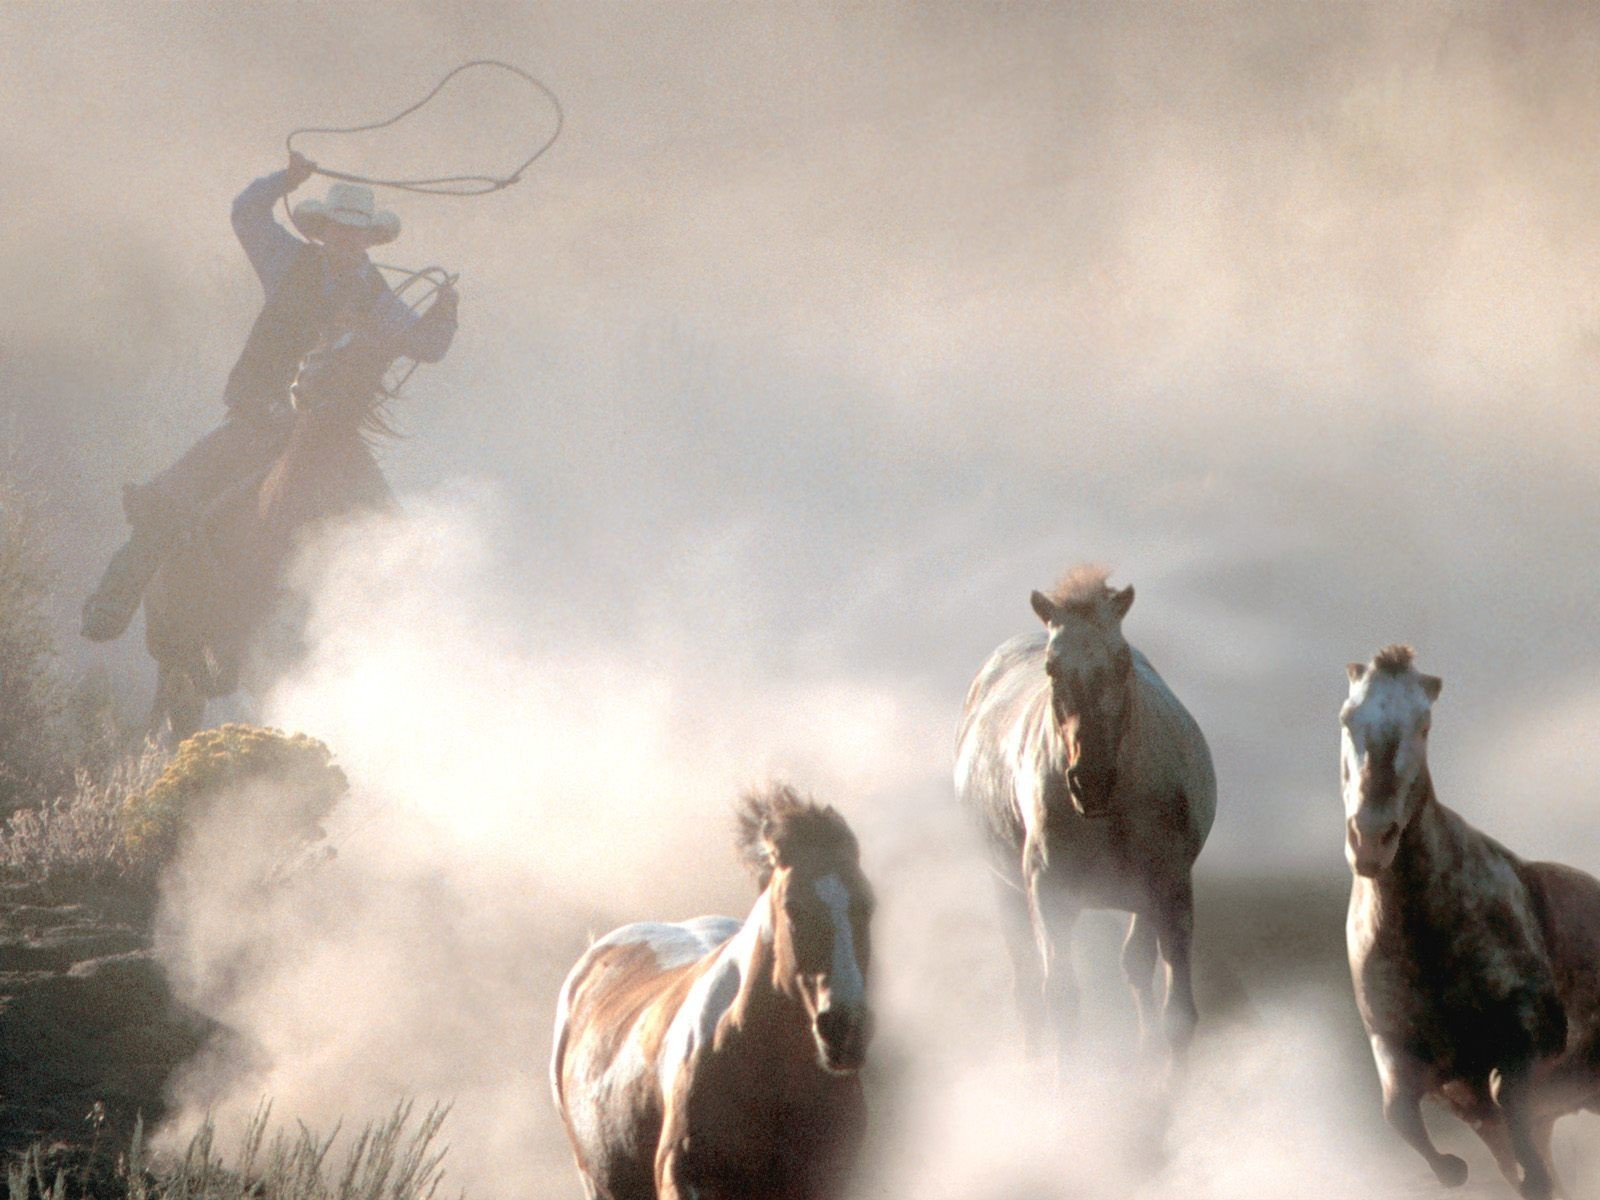
\includegraphics[width=\paperwidth]{wrangle.jpg}}%
% OPTIONAL TITLE PAGE SLIDE----------------
\begin{frame}

\titlepage % Print the title page as the first slide

\end{frame}
}



% OPTIONAL TABLE OF CONTENTS SLIDE---------

\begin{frame}
\frametitle{Overview} % Table of contents slide, comment this block out to remove it
\tableofcontents % Throughout your presentation, if you choose to use \section{} and \subsection{} commands, these will automatically be printed on this slide as an overview of your presentation
\end{frame}

% OPTIONAL SECTION HEADERS-----------------
\section{First Section} % Sections can be created in order to organize your presentation into discrete blocks; all sections and subsections are automatically printed in the table of contents as an overview of the talk

\subsection{Subsection Example} % A subsection can be created just before a set of slides with a common theme to further break down your presentation into chunks

% SLIDE (BULLET POINTS)--------------------
\begin{frame}
\frametitle{Bullet Points}
\begin{itemize}
\item first item
\item second item
\item third item
\item et cetera
\item last item
\end{itemize}
\end{frame}

% SLIDE (SEQUENTIAL BULLET POINTS)---------
\begin{frame}
\frametitle{Sequential Bullet Points}
\begin{itemize}
\item<1-> Text visible on first slide
\item<2-> Text visible on second slide
\item<3-> Text visible on third slide
\end{itemize}
\end{frame}

% SLIDE (FIGURE)-----------------------------
\begin{frame}
\frametitle{Figure}
% Uncomment the code on this slide to include your own image from the same directory as the template  file.
% \begin{figure}
% use this format for absolute sizing
%\includegraphics[width=3cm, height=4cm]{filename.jpg}
% \end{figure}
\end{frame}

% SLIDE (TABLE)----------------------------
\begin{frame}
\frametitle{Table}
\begin{table}
\begin{tabular}{l l l}
\toprule
\textbf{Treatments} & \textbf{Response 1} & \textbf{Response 2}\\
\midrule
Treatment 1 & 0.0003262 & 0.562 \\
Treatment 2 & 0.0015681 & 0.910 \\
Treatment 3 & 0.0009271 & 0.296 \\
\bottomrule
\end{tabular}
\caption{Table caption}
\end{table}
\end{frame}

%------------------------------------------------
\section{Second Section}
%------------------------------------------------
% SLIDE (PARAGRAPHS OF TEXT)---------------
\begin{frame}
\frametitle{Paragraphs of Text}
Sed iaculis dapibus gravida. Morbi sed tortor erat, nec interdum arcu. Sed id lorem lectus. Quisque viverra augue id sem ornare non aliquam nibh tristique. Aenean in ligula nisl. Nulla sed tellus ipsum. Donec vestibulum ligula non lorem vulputate fermentum accumsan neque mollis.\\~\\

Sed diam enim, sagittis nec condimentum sit amet, ullamcorper sit amet libero. Aliquam vel dui orci, a porta odio. Nullam id suscipit ipsum. Aenean lobortis commodo sem, ut commodo leo gravida vitae. Pellentesque vehicula ante iaculis arcu pretium rutrum eget sit amet purus. Integer ornare nulla quis neque ultrices lobortis. Vestibulum ultrices tincidunt libero, quis commodo erat ullamcorper id.
\end{frame}

% SLIDE (BLOCKS OF HIGHLIGHTED TEXT)-------
\begin{frame}
\frametitle{Blocks of Highlighted Text}
\begin{block}{Block 1}
Lorem ipsum dolor sit amet, consectetur adipiscing elit. Integer lectus nisl, ultricies in feugiat rutrum, porttitor sit amet augue. Aliquam ut tortor mauris. Sed volutpat ante purus, quis accumsan dolor.
\end{block}

\begin{block}{Block 2}
Pellentesque sed tellus purus. Class aptent taciti sociosqu ad litora torquent per conubia nostra, per inceptos himenaeos. Vestibulum quis magna at risus dictum tempor eu vitae velit.
\end{block}

\begin{block}{Block 3}
Suspendisse tincidunt sagittis gravida. Curabitur condimentum, enim sed venenatis rutrum, ipsum neque consectetur orci, sed blandit justo nisi ac lacus.
\end{block}
\end{frame}

% SLIDE (EMBEDDED R CODE)------------------
\begin{frame}[fragile]{Embedded R Code; \texttt{fragile} frame}
\begin{block}

\begin{knitrout}
\definecolor{shadecolor}{rgb}{0.969, 0.969, 0.969}\color{fgcolor}\begin{kframe}
\begin{alltt}
\hlcom{# show some output...}
\hlkwd{runif}\hlstd{(}\hlnum{10}\hlstd{)}
\end{alltt}
\begin{verbatim}
##  [1] 0.13279632 0.15808441 0.79218866 0.22428359 0.84602719 0.04939383
##  [7] 0.10616781 0.33116594 0.61229214 0.20378845
\end{verbatim}
\end{kframe}
\end{knitrout}

\end{block}
\end{frame}

% SLIDE (EMBEDDED R FIGURE)----------------
\begin{frame}[fragile]{Embedded R Figure; \texttt{fragile} frame}
%\begin{block}

\begin{knitrout}
\definecolor{shadecolor}{rgb}{0.969, 0.969, 0.969}\color{fgcolor}

{\centering 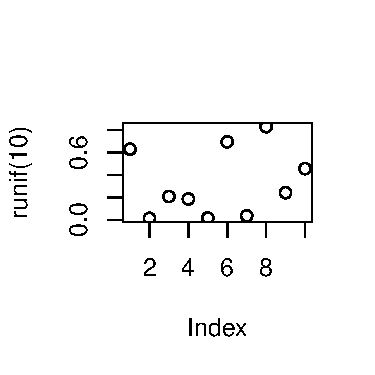
\includegraphics[width=\maxwidth]{figure/unnamed-chunk-2-1} 

}



\end{knitrout}

%\end{block}
\end{frame}

% SLIDE (MULTIPLE COLUMNS)-----------------
\begin{frame}
\frametitle{Multiple Columns}
\begin{columns}[c] % The "c" option specifies centered vertical alignment while the "t" option is used for top vertical alignment

\column{.45\textwidth} % Left column and width
\textbf{Heading}
\begin{enumerate}
\item Statement
\item Explanation
\item Example
\end{enumerate}

\column{.5\textwidth} % Right column and width
Lorem ipsum dolor sit amet, consectetur adipiscing elit. Integer lectus nisl, ultricies in feugiat rutrum, porttitor sit amet augue. Aliquam ut tortor mauris. Sed volutpat ante purus, quis accumsan dolor.

\end{columns}
\end{frame}


% SLIDE (THEOREM)----------------------------
\begin{frame}
\frametitle{Theorem}
\begin{theorem}[Mass--energy equivalence]
$E = mc^2$
\end{theorem}
\end{frame}

% SLIDE (VERBATIM)---------------------------
\begin{frame}[fragile] % Need to use the fragile option when verbatim is used in the slide
\frametitle{Verbatim}
\begin{example}[Theorem Slide Code]
\begin{verbatim}
\begin{frame}
\frametitle{Theorem}
\begin{theorem}[Mass--energy equivalence]
$E = mc^2$
\end{theorem}
\end{frame}\end{verbatim}
\end{example}
\end{frame}

% SLIDE (FINAL SLIDE)------------------------
\begin{frame}
\Huge{\centerline{The End}}
\end{frame}

%------------------------------------------------
\end{document}
